\documentclass[12pt]{article}
 \usepackage[hcentering,bindingoffset=20mm]{geometry}
 \usepackage{placeins}
 \usepackage[numbib]{tocbibind}
 \usepackage{rotating}
\usepackage[square,sort,comma,numbers]{natbib}
 \usepackage{graphicx}
 \usepackage{tabularx}
% \usepackage{datetime2}
 \linespread{1.3}
 \usepackage{gensymb}
\usepackage{longtable}
 \usepackage{lscape}
 \usepackage{url}
 \addtolength{\textwidth}{2cm}
 \addtolength{\hoffset}{-1cm}
 
 
 \addtolength{\textheight}{2cm}
 \addtolength{\voffset}{-1cm}
 \setlength{\parindent}{0pt}
 

\title{Trial by phylogenetics - how model and data selection impacts the elucidation of the evolution of the Gonyaulacales (Dinophyceae). $^{1}$}
\author{Key words: Bayesian inference, model selection, Gonyaulacales, phylogenetics, transcriptomics}

\date{}

\begin{document}
\maketitle

%Timestamp \DTMnow UTC %sorry for some reason datetime2 package is breaking the rendering process - the tracklang dependency got updated or something and it's throwing a hissy fit. After about an hour of trying to fix it, I think I should be looking at the manuscript instead =\

\paragraph{}Anna Liza Kretzschmar$^{2}$\\
Climate Change Cluster (C3), University of Technology Sydney, Ultimo, 2007 NSW, Australia, anna.kretzschmar@uts.edu.au
\paragraph{}Aaron E. Darling \\
The ithree institute, University of Technology Sydney, Ultimo, 2007 NSW, Australia
\paragraph{}Mathieu Fourment \\
The ithree institute, University of Technology Sydney, Ultimo, 2007 NSW, Australia
\paragraph{}Arjun Verma\\
Climate Change Cluster (C3), University of Technology Sydney, Ultimo, 2007 NSW, Australia
\paragraph{}Shauna Murray\\ 
Climate Change Cluster (C3), University of Technology Sydney, Ultimo, 2007 NSW, Australia
\newpage
\section{Abstract}
\newpage

\section{Introduction}
Historically, the limiting factor for phylogenetics has been availability of genetic data to infer evolutionary relationships.
Now, the breadth of publicly available datasets generated by high throughput sequencing techniques allow for an increasingly detailed investigation into the evolutionary relationships between organisms.
The quest to untangle the relationships within the evolutionary tree is an ongoing process that can help inform a broad range of fields, for example epidemiology, toxicology and ecological interactions \cite{mctavish2017and}. %sm: arbitrary list needs to be comprehensive %LK: better?
% AD: also, i'm not sure what the 2nd half of this sentence means. suggest splitting it into its own sentence(s) and try to improve clarity by rephrasing. LK: better?
A limiting factor for our analysis of evolutionary relationships is, commonly, the computational methods and available infrastructure used to analyze the datasets. 
Another is that the methods and models applied to the dataset can influence the resulting phylogeny and there needs to be a solid understanding of the methods, including their shortcomings, by the operator.
An example of the breadth of publicly available data is the Marine Microbial Eukaryote Transcriptome Sequencing Project (MMETSP), which sequenced transcriptomes of over 650 marine eukaryotic microbes \cite{keeling2014marine}. 
This project focused on a group of understudied organisms which are abundant and play vital roles in the marine environment, from geochemical cylcling, predation to symbiosis. %sm: ref
This dataset offers an excellent opportunity to explore the evolutionary relationships between these taxa through phylogenetics. 
For phylogenetic inference, the gene representative for each taxa is compared with all other representatives. 
The assumption for an accurate representation of species evolution is based on this gene comparison using genes that diverged strictly through  gene tree divergence due to speciation (= orthology) rather than duplication (= paralogy) or transfer from another organism (= horizontal gene transfer) \cite{maddison1997gene}. 
Both paralogs and orthologs are specific cases of homology, genes which share an ancestral sequence and diverged in the past, where the mode of divergence differs \cite{fitch1970distinguishing}. 
The distinction between these two cases is essential in identifying gene candidates that are informative for species evolution inference, as the selection of orthologs ensures the inclusion of a signal that is based on the speciation of the taxa examined, while selection of paralogs confounds that signal by including information that does not pertain to the speciation of the taxa. 
As gene loss and duplication can commonly occur in a number of the lineages examined, the establishment of orthology is more difficult than may seem apparent from the definition \cite{gabaldon2008large}. 
Once orthologs are selected, there are further issues that can arise and impact the veracity of the phylogenetic inference. 
Two common, well characterized types of errors are random (sampling) and systematic errors. 
The former arises from the data, as individual gene histories may differ to the species tree. 
With a small number of genes, this random error can skewer the inference results away from the true species tree, however increasing the number of genes directly reduces the impact this error has on the analysis. 
Conversely, systematic errors arise due to the mispecification of the model used for the inference where an incorrect species tree topology results. 
In this case, an increase in dataset size can exacerbate systematic error rather than reduce it as would happen with random errors (see Box 1). 
In the presence of this type of systematic error, the resulting inference can be positively misleading,
 with high clade support values for the incorrect tree topology, obfuscating the presence of the error \cite{jeffroy2006phylogenomics,roch2015likelihood,kubatko2007inconsistency}. 
Common problems in carrying out a species tree inference arise from:\\
1) Selection of paralogs. 
If genes with different evolutionary histories are selected, the gene tree will not reflect the history of either paralog and be nonsensical for species tree inference; \\
2) Concatenation of genes. 
Can be statistically inconsistent estimator of the species tree due to incomplete lineage sorting and concatenation acting as imperfect estimator of species tree topology \cite{roch2015likelihood}; and \\
3) Inference of model adequacy from bootstrap values. 
Kubatko et al. (2007) demonstrated high bootstrap support under maximum likelihood (ML) inference for incorrect species trees with concatenated gene sets as input \cite{kubatko2007inconsistency}. 
As high bootstrap values are often used as an indicator for robust species topology resolution, this fallacy is particularly problematic if the reader/operator is unfamiliar with the statistical phenomenon.\\
In this study we aim to demonstrate a bioinformatic methodology which attempts to mitigate the effects of paralogy when processing transcriptomic data than currently commonly utilized in protistology. 
Further, we seek to demonstrate the impact of model and data selection on the resulting phylogenetic inference. 
We provide open source scripts to assemble RNA-seq datasets, identify and extract single copy genes across input taxa with extensive paralogy, and aligns selected genes ready for Bayesian inference (BI) phylogenetics. 
%AD: can you give the URL for script download? e.g. the github repo?
%LK: should I do this here or in the methods?
Finally, the methodology is tested with a group of organsims notorious for their extensive paralogy - the Gonyalacales (phylum: Dinoflagellata) (see box 2 for further information on the Gonaylacales).
%need: limited taxon sampling
\subsubsection*{Box 1: Statistical nomenclature \& errors this study seeks to address}
For in depth explanations see \cite{yang2014molecular}.\\
\textbf{Bayesian probability (BI):} infers posterior probability from expectation based prior probability compared to data based likelihood function which assesses the differences in prior and likelihood of each parameter.
BI uses probability distributions to describe uncertainty in parameters.
Model re-parameterization via priors changes posterior output, i.e. this is a dynamic method informed by observation as input by the user. 
We recommend Huelsenbeck et al. (2001) for an overview of the principles underlying BI for phylogenetics \cite{huelsenbeck2001bayesian}.\\
%AD: i'm not sure what the following two sentences mean. it doesn't sound right.
%LK: is this a clearer explanation of MLE?
\textbf{Maximum likelihood estimate (MLE):} estimates the values for the parameters of the model that maximise the likelihood of the result given the observed data. 
The likelihood is invariant to re-parameterization as the most likely values for the parameters are not affected, so where a change in prior designation would affect Bayesian probability, this would not affect MLE.
Does not use priors, which means probability functions not applied to model parameters, but only their estimates. 
Model reparameterization does not affect MLE, in effect a static method.\\
\textbf{Heterotachy:} change in evolutionary rates of sites over time, specific to lineage(s).\\
\textbf{Potential statistical error types:}\\
1. random. Sampling based error which decreases and approaches zero as size of dataset approaches infinity.\\
2. systematic. Arises from incorrect model assumptions or problems with the model itself. 
Error type persists and increases as dataset size approaches infinity. 
If strong, can override true phylogenetic signal.\\
\textbf{Incomplete lineage sorting:} discordance of gene evolutionary history with the species evolutionary history causing the phylogenetic species tree to be misinfered. 
Difference in the topology of a gene tree compared to the species evolution can arise from the coalescence of those orthologs pre-dating the species divergence, in effect having an ancestral state where several copies of the gene were present in the population for one or more species divergence points. 
Another mechanism is the introduction of a copy of the gene which is not based on ancestral inheritance, such as horizontal gene transfer or hybridization.\\
\textbf{Long branch attraction:} phylogenetic phenomenon where distantly related taxa are inferred as close relatives topologically due to systematic error, also known as the Felsenstein zone.

\subsubsection*{Box 2: Who/what are the Gonyaulacales?}
%TODO Aaron and Mathieu, as non protistologists is this section adequate in explaining why the gonyaulacales were chosen for this work, or would it help to include some of the commented out text?
The Gonyaulacales are an order within the super-phylum Alveolata and sub-phylum Dinoflagellata, which are an ancient lineage on the eukaryotic branch of life \cite{moldowan1998biogeochemical}. 
They play a role in several important ecological processes in aquatic environments where they cover a diverse array of niches such as symbionts, parasites and autotrophs. 
Some taxa can cause harmful algal blooms through proliferation and/or neurotoxin production (e.g. causing paralytic shellfish poisioning, ciguatera fish poisoning) \cite{murray2016unravelling}.
Dinoflagellates possess large genomes (estimated 3.7 to 220 Gbp), with extensive paralogy and repetitive short sequences  \cite{casabianca2017genome,murray2016unravelling}. 
In particular the paralogy has proven problematic for efforts investigating the genetic content and structure of the dinoflagellates, as this feature has prevented the assembly of genomes apart from two draft genomes for \textit{Symbiodinium} which posess some of the smaller genomes 
cite{shoguchi2013draft,lin2015symbiodinium}. 
For a review on the genetic features of dinoflagellates see \cite{murray2016unravelling}. 
While the evolutionary relationship of most orders within the dinoflagellates has been inferred with consistently high support values, one order has often escaped elucidation - the Gonyaulacales. 
%Analyses for this order commonly combined concatenation and maximum likelihood approaches, which yielded long branch attraction, low confidence values and inconsistent taxon resolution \cite{}. 
As neurotoxin production is prevalent in this order, the evolution of the order is of interest to give a a base line for investigating how the toxins evolved \cite{shalchian2006combined,zhang2007three,saldarriaga2004molecular,hoppenrath2010dinoflagellate,murray2005improving}. 
%Specifically the ciguatoxins produced by some \emph{Gambierdiscus} spp. are of interest as the causative agent of ciguatera fish poisoning, a neglected tropical disease with global implications \cite{globalcig}.%, which is predicted to increase in prevalence as climate change progresses \cite{}.

\newpage
\section{Materials and methods}
\subsection*{Culture conditions}
\FloatBarrier
Cultures were isolated from locations as per Table S1 and clonal cultures established by micropipetting single cells through sterile seawater. 
Clonal cultures were maintained in F/10 medium and maintained at temperatures indicated in Table S1. 

\subsection*{RNA isolation}
\emph{Gambierdiscus} spp. and \emph{Thecadinium} cf. \emph{kofoidii} were harvested during late exponential growth phase by filtration onto 5 $\mu$m SMWP Millipore membrane filter (Merck, DE) and washed off with sterile seawater. 
Cells were pelleted via centrifugation (make of centrifuge) for 10 minutes at 350 rcf. 
Supernatant was decanted and 2ml of TRI Reagent (Sigma-Aldrich, subsidiary of Merck, DE) was added to the pellet and vortexed till dissolved. 
Samples were split in two and transferred to 1.5ml eppendorf tubes. 
Cellular thecae were ruptured by three rounds of freeze-thaw, with tubes transferred between liquid Nitrogen and 95 $^{\circ}$C. 
RNA was extracted as per protocol for TRI Reagent. 
RNA elute was purified with the RNeasy RNA clean up kit EXACT NAME as per protocol(Qiagen). 
DNA was digested with TurboDNAse (Life technologies, subsidiary of Thermo Fischer scientific, AU). 
RNA was quantified with Nanodrop 2000 (Thermo Scientific, Australia) and frozen at -80 $^{\circ}$C until sequencing.
%TODO insert centrifuge, kit name deets
 
\subsection*{Library preparation and Sequencing}
The quality of samples was assessed via an Agilent 2100 Bioanalyzer. 
Paired-end sequencing was performed with a NextSeq 500 High Output run at the Ramaciotti Centre (UNSW, AU) with 75bp read lenth for \emph{G. lapillus} and \emph{G.} cf. \emph{silvae}; and 150bp read length for \emph{G. carpenterii}, \emph{G. polynesiensis} CG15 and \emph{T.} cf. \emph{kofoidii}.

\subsubsection*{Publically available transcriptome libraries}
The \emph{Gambierdiscus excentricus} VGO790 transcriptome was downloaded from NCBI under accession ID SRR3348983 \cite{kohli2017role}. 
\textit{Coolia malayensis}, \textit{Ostreopsis ovata}, \textit{Ostreopsis rhodesae} and \textit{Ostreopsis siamensis} transcriptomes were supplied by Arjun Verma (Verma 2018, in prep). 
RNA seq libraries for all remaining transcriptomes were generated by, and downloaded from, the Marine Microbial Eukaryote Transcriptome Sequencing Project \citep{keeling2014marine}.

\subsection*{Transcriptome processing scripts}
The analysis workflow was written in the Nextflow language \cite{nextflow} for streamlined transfer between high performance computing clusters and is available on Github under hydrahamster/gonya\_phylo. 
The workflow is separated into two parts, and modules within the scripts are written in bash and Python 2.7 \cite{python}, including the pandas module \cite{pandas}, and can be found on Github. 
Our datasets were analysed using a Genomics Virtual Lab (GVL) \cite{afgan2015genomics} instance in the NeCTAR cloud.
\subsubsection*{Transcriptome assembly}
Individual RNA sequencing libraries are the input, which are then processed through FastQC \cite{fastqc} for quality metrics, sequences are trimmed with Trimmomatic (LEADING:3 TRAILING:3 SLIDINGWINDOW:4:5 MINLEN:25) \cite{bolger2014trimmomatic} and assembled with Trinity v2.4.0 (default settings for paired end libraries) \cite{haas2013novo}. 
Assemblies were then processed with BUSCOv2 with the protist specific library \cite{simao2015busco}.
The RNA libraries with 150bp reads generated as part of this study were also subjected to Digital Normalization \cite{diginorm} prior to assembly, to pool identical transcripts before assembly which were then used for downstream analysis.                                                                                                                                                                                                                                                                                                                                                                                                                                                                                                                                                                                                                                                                                                                                                                                                                                                                                                                                                                                                                                                                                                                                                                                                                                                                                                                                        
\subsubsection*{Construction of multiple alignments}
The BUSCOv2 output from all transcriptomes from the previous step forms the input for identification of single copy genes and construction of multiple alignments. 
Any genes that were present as single copies in at least 75 \% of the transcriptomes were indexed, the corresponding contig extracted from the assemblies, aligned with hmmer3.1b2 \cite{eddy2015hmmer} and unaligned regions trimmed.
If several candidate sequences are processed for the same organism, a warning message in the command interface alerts the user before proceeding. 
The output for this section was used as basis for single copy gene phylogenetic inferences in subsequent sections.

\subsection*{Assembly analysis}
Contigs from assemblies were clustered with cd-hit with the flags T 10 -M 5000 -G 0 -c 1.00 -aS 1.00 -aL 0.005 \cite{fu2012cd}. 
Protein coding regions were predicted with Transdecoder \cite{haas2016transdecoder}.
Amino acid clusters were clustered again with cd-hit with the flags as previously except -c 0.98.
Protein sequences were analysed with interproscan v5.27 with local lookup server \cite{quevillon2005interproscan}.

\subsection*{Phylogenetic inferences}
\subsubsection*{Ribosomal DNA based inference}
Ribosomal DNA (rDNA) sequences for the small subunit (SSU) region as well as the D1-D3 large subunit (LSU) region were acquired from NCBI \cite{coordinators2017database} or the SILVA rRNA database project \cite{silvaproj}, accession IDs in Table S3. 
%AD: I guess these didn't go through infernal?
%LK: no they did not. That inquiry was for a side project
Individual genes were aligned using the MUSCLE algorithm a maximum of 8 iterations \cite{edgar2004muscle}, then were concatenated in Geneious v11.3 \cite{kearse2012geneious}.
ML inference was obtained using RaxML \cite{stamatakis2014raxml} with the GTR and GAMMA flags, with 100 bootstraps.

\subsubsection*{Concatenated single copy gene based inference}
Single copy gene alignments were concatenated and both ML \& BI analyses were executed on the University of Technology Sydney's High-performance computing cluster (HPCC). 
GPU processing units were either Nvidia Tesla K80 or a Tesla P100. 
\paragraph*{Maximum likelihood with concatenated sequences.}
ML inference run as described in the previous section, with the ILGF, GAMMA and PROT flags.
\paragraph*{Bayesian inference with concatenated sequences.}
BI was run in BEAST2 with the Gamma site model with 4 Gamma category counts under the WAG substitution model \cite{whelan2001general}. A local random clock was used  under the Birth Death model %TODO insert nuber of chains etc
 

\paragraph*{Bayesian probability under the multispecies coalescent.}
Bayesian inference of the species tree was carried out under the *BEAST2 model in BEAST2 \cite{bouckaert2014beast}. 
The analysis was performed with the WAG amino acid substitution model \cite{whelan2001general} and with a Gamma distribution for four rate categories. 
A random local clock was employed \cite{drummond2010bayesian}. 
Inference was executed on the HPCC. 
Inference was accelerated using BEAGLE \cite{ayres2011beagle} on the GPU. 
Posterior distributions of parameters were approximated after 300,000,000 generations of MCMC runs, sampled every 5,000 generations with a burn in of 15\%. 
The inference was run four times to compare convergence of parameters, then log and tree files were merged. 

%\subsection*{stepping stone analysis}
%TODO put details in in the distant future

\subsection*{Inference run time comparison}
A subset of 14 taxa was selected for a comparison between CPU and GPU inference run time comparison. 
The transcriptome libraries were fed through the single copy gene extraction script as described, which was set to extract single copy genes present in all of the taxa. 
The resulting alignments were run on *BEAST either on the CPU or GPU.

\subsubsection*{Generation of figures}
Tanglegrams were generated with Dendroscope v3.5.9 \cite{huson2007dendroscope}; images were edited in GIMP \cite{gimp}.
\newpage
\section{Results}
\subsection*{Transcriptomes overview}
RNA-sequencing libraries generated in this study are available on NCBI's sequence read archive under the project ID SRP134273.
Sequencing of transcriptomes for \emph{Gambierdiscus} spp. and \emph{T.} cf. \emph{kofoidii} generated datasets ranging in size from, 143,155,667 to 233,822,334 reads, resulting in 97,634 to 191,224 assembled contigs (table ~\ref{tbl:asmstats}). 
Clusters with gene ontology (GO) annotations made up 30.9\% to 34.8\% of the total clusters. 

\FloatBarrier
\begin{longtable}{  | p{3cm} |p{2.2cm} | p{2.2cm} | p{2.2cm} | p{2.2cm} | p{2.2cm} |}
\caption{Summary of transcriptome sequencing and assembly statistics.}\\
\hline
\label{tbl:asmstats}
\emph{Sequences:}&\emph{G. carpenteri}&\emph{G. lapillus}&\emph{G. polynesiensis}&\emph{G.} cf. \emph{silvae}&\emph{T.} cf. \emph{kofoidii}\\
\hline
 \multicolumn{6}{| c |}{Sequencing}\\
 \hline
\textbf{SRA accession}&SRR6821720&SRR6821722&SRR6821723&SRR6821721&SRR6821724\\
\hline
\textbf{Raw sequencing reads}&186,422,744&145,366,966&217,031,342&143,155,667&233,822,334\\
\hline
%\textbf{Size (Gb)}&16.92&&19.51&&21.08\\
%\hline
 \multicolumn{6}{| c |}{Assembly}\\
 \hline
 \textbf{Contigs \#}&105,464&148,972&114,622&191,224&97,634\\
\hline
\textbf{Average length (bp)}&607&1,139&633&953&581\\
%\hline
%\textbf{Minimum length (bp)}&201&201&201&201&201\\
\hline
\textbf{Maximum length (bp)}&7,448&12,370&6,608&8,198&7,922\\
\hline
  \multicolumn{6}{| c |}{Transcript clustering \& annotation}\\
\hline
\textbf{\# clusters}&139,699&92,418&139,487&107,766&116,468\\
\hline
\textbf{Contigs with GO annotations}&44,167&32,140&43,098&34,201&37,656\\ %cut -f 3 my.gff | sort | uniq | wc -l .. maybe diff to '3' but hey
\hline
%\textbf{with full annotations}&&&&&\\
%\hline
%\textbf{with Enzyme Codes}&&&&&\\
%\hline
%\textbf{mapped to KEGG pathways}&&&&&\\
%\hline
\end{longtable}

\subsection*{BUSCO output}
Assemblies were searched with BUSCOv2 and the single copy genes were extracted. 
The single copy genes acquired though the BUSCO HMMER libraries curated for protists are reported in Table S2 out of the total 234 genes searched for, as well as accession numbers and identifiers for each transcriptome. 
%AD: good idea to post to zenodo //LK:  thanks ^__^
Single copy genes for each transcriptome used in this study are available on Zenodo DOI:
%TODO single copy genes need ot go up on Zenodo, then link DOI here

\subsection*{Phylogenetic inferences}
Support for branches was interpreted as follows, for ML and BI, respectively: 100\%/1.0 was considered fully supported, above 90\%/0.9 was very well supported, 80\%/0.8 and above was interpreted as relatively well supported and above 50\%/0.5 was considered weakly supported but below was considered unsupported.
As \emph{Azadinium spinosum}, \emph{Dinophysis acuminata} and \emph{Karenia brevis} are members of different orders (Dinophyceae ordo incertae sedis, Dinophysiales \& Gymnodiniales respectively) and consistently resolve outside of the Gonyaulacales in phylogenetic analyses, their placement as an outgroup was considered a given for this study. 
%sm:what about crypthecodinium
%LK: that genus has been routinely placed within the gonyaulacales incl on reference databases like NCBI, encyclopedia of life so it's placement as outgroup is not a given and uncertain at best
Hence the unifying branch for these taxa was used to root the tree in all subsequent analyses.
\subsubsection*{rDNA based phylogeny}
\FloatBarrier 
All nodes were supported, with a range of certainty.
The following refers to Fig. ~\ref{fig:rdna}.
Species within the genera \emph{Gambierdiscus} and \emph{Ostreopsis} resolved with their sister species with full support. 
Within the \emph{Gambierdiscus} clade, nodes are either weakly supported or fully supported. 
The two species of \emph{Alexandrium} resolve as well supported closest relatives, but do not form an individual clade. 
%AD: crown taxa is a new one for me - surprising after 15 years thinking about phylogeny!
%LK: That's a good thing, right?
Deeper nodes were supported but with less certainty than the crown taxa. 
Two distinct clades can be observed from the topology: One including \emph{Alexandrium}, \emph{Coolia} and \emph{Ostreopsis}; another with only \emph{Gambierdiscus}. 
Sister to these clades, in descending order, was \emph{Pyrodinium}, \emph{Ceratium} and \emph{Gonaulax}, \emph{Protoceratium} and \emph{Thecadinium}. 
The outgroup was relatively well supported and included \emph{Crypthecodinium}. 
Support for deeper nodes varied from weak to well supported.

\begin{figure} 
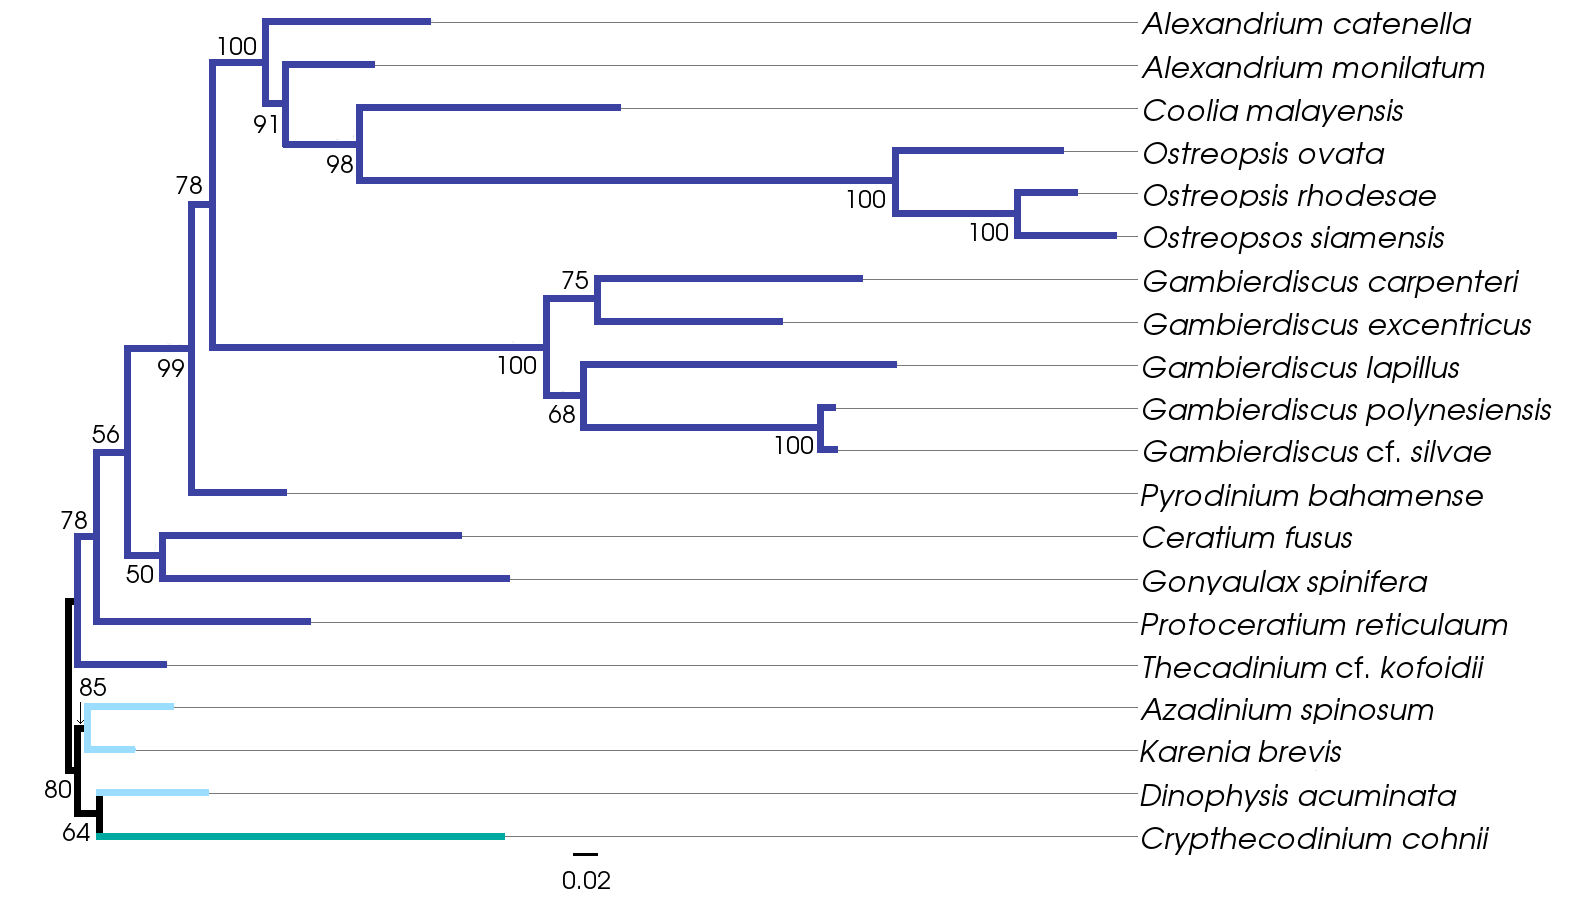
\includegraphics[scale=.4]{figures/rDNA-ML.png} 
\caption{Maximum likelihood phylogenetic inference of ribosomal DNA genes. Concatenation of small subunit rDNA and D1-D3 region large subunit rDNA. Accession numbers for concatenated genes in Table S3. Gonyaulacales (\#16) in purple, outgroups (\#3) in light blue and taxa \textit{incertae sedis} (\#1) in teal. The scale represents number of substitutions per site.} 
\label{fig:rdna}
\end{figure} 
\FloatBarrier

\subsubsection*{Concatenated single copy gene based phylogeny inferred with ML}
\FloatBarrier
All nodes except one within the \emph{Gambierdiscus} species cluster resolved as relatively well supported. 
Topological description in this section refers to Fig. ~\ref{fig:SCconcatML}. 
Species of the genera \emph{Alexandrium}, \emph{Gambierdiscus} and \emph{Ostreopsis} cluster as individual clades with their sister species.  
The topology shows three distinct, well supported clades: 
One encompassing \emph{Alexandrium}, \emph{Coolia} and \emph{Ostreopsis}; another which only contains \emph{Gambierdiscus}; and one which includes \emph{Pyrodinium}, \emph{Gonyaulax} and \emph{Protoceratium}. 
Sister to these clades is \emph{Thecadinium}, followed by \emph{Ceratium}. .
The split of the outgroup was fully supported, while the internal nodes resolved very well supported. 
\emph{Crypthecodinium} resolved within the outgroup, sister to \emph{Karenia}. 
Other deeper nodes were well supported.
 
\begin{figure} 
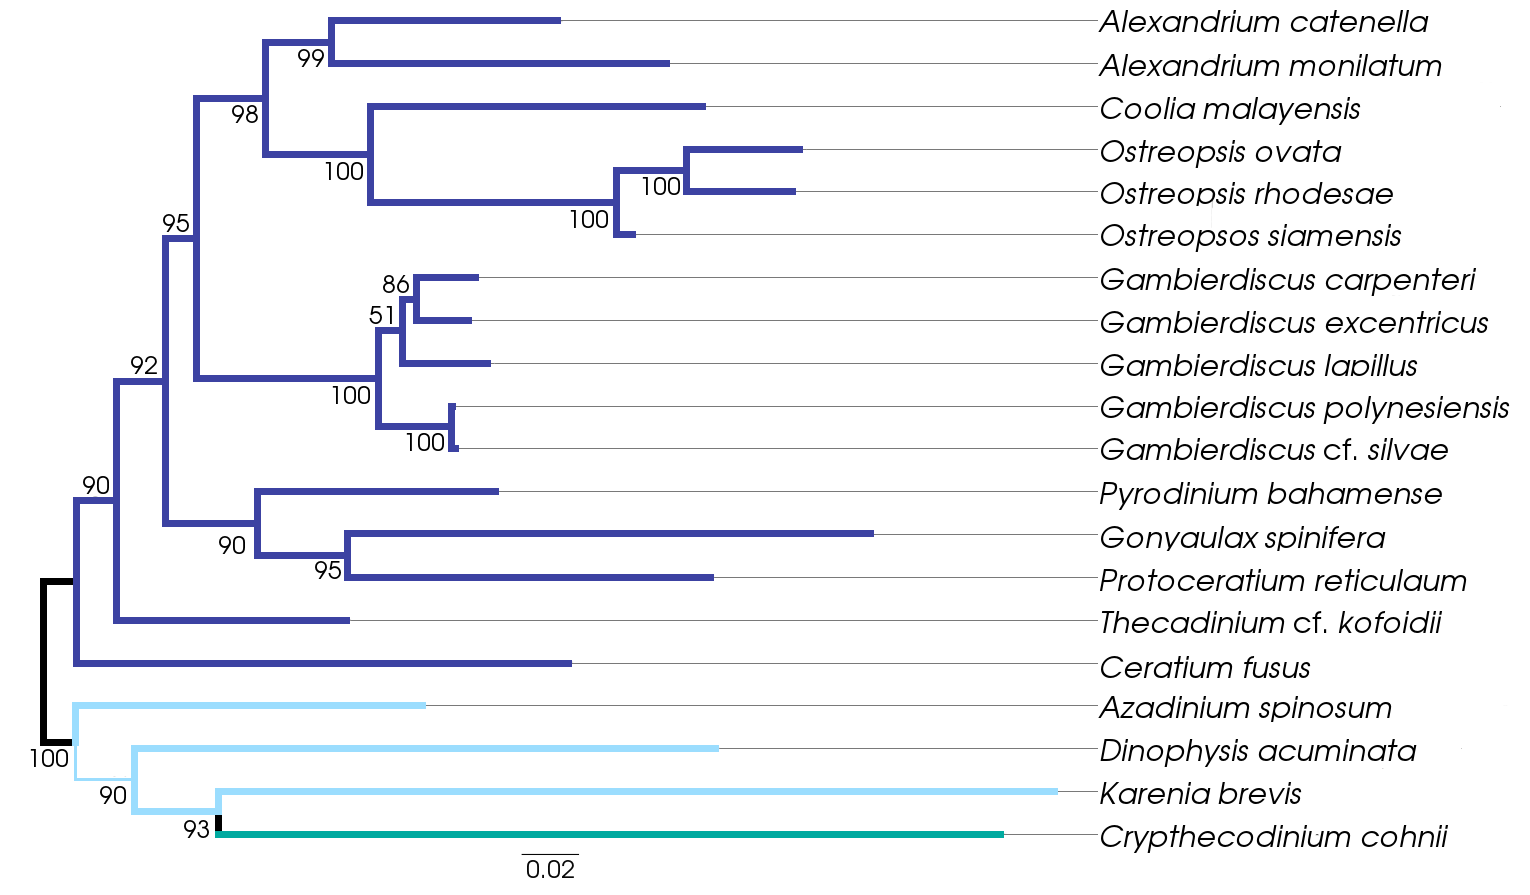
\includegraphics[scale=.45]{figures/Singlecopy-concat-ML.png} 
\caption{Maximum likelihood phylogenetic inference of concatenated single copy gene set (62 single copy genes from 20 taxa). Gonyaulacales (\#16) in purple, outgroups (\#3) in light blue and taxa \textit{incertae sedis} (\#1) in teal. The scale represents number of substitutions per site.} 
\label{fig:SCconcatML}
\end{figure} 
\FloatBarrier

\subsubsection*{Concatenated single copy gene based phylogeny inferred with BI}
\FloatBarrier 
%TODO Running with stepping stone ~~~ check out trees closer to posterior for prev ss sampling run in /shared/homes/s1/Liza/concat-bollocks/test
All nodes resolved with full support, except one node within the genus \textit{Gambierdiscus} which was very well supported. 
The following descriptions are based on Fig. ~\ref{fig:SCconcatBI}. 
The species in the genera \textit{Alexandrium}, \textit{Gambierdiscus} and \textit{Ostreopsis} all resolved with full support within their respective genera clades. 
The overall topology of the Gonyaulacales resolved as three clades with \textit{Thecadinium} and then \textit{Ceratium} as ancestral lineages. 
\textit{Alexandrium}, \textit{Coolia} and \textit{Ostreopsis} clustered together, followed by \textit{Gambierdiscus} on their own in a sister clade. 
The third clade encompasses \textit{Gonyaulax}, \textit{Protoceratium} and \textit{Pyrodinium}. 

\begin{figure} 
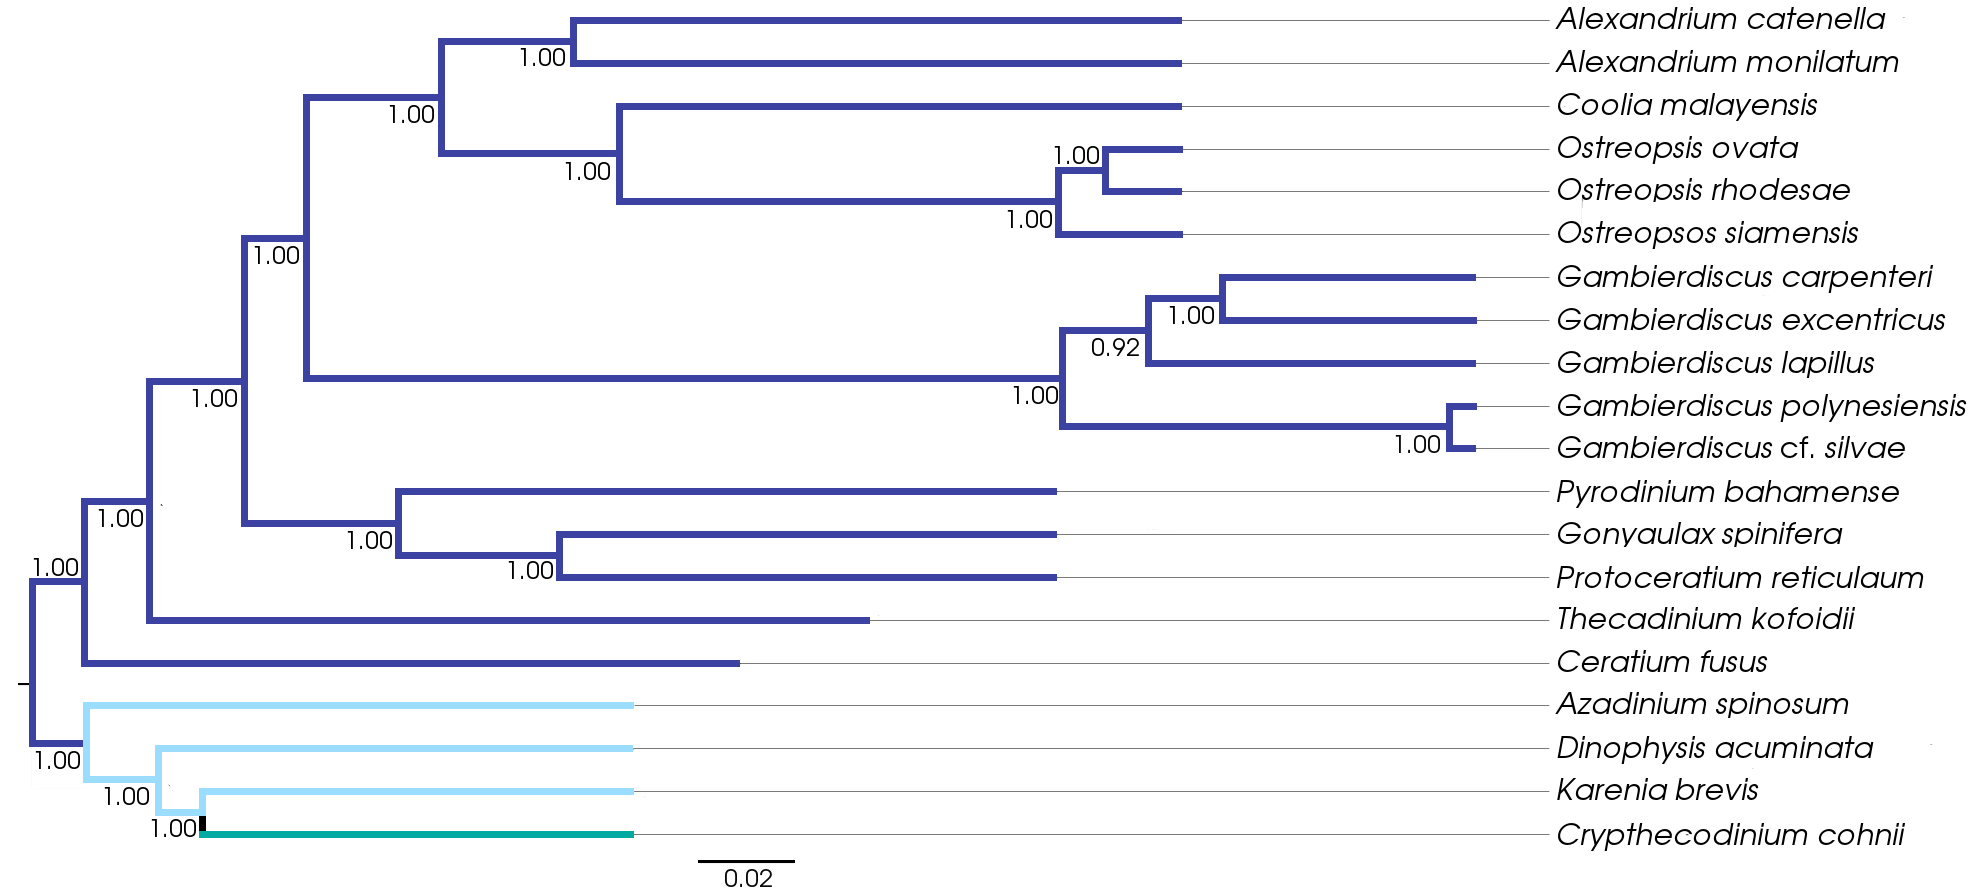
\includegraphics[scale=.3]{figures/SC-concat-BI.png} 
\caption{Bayesian phylogenetic inference of concatenated single copy gene set (62 single copy genes from 20 taxa). Gonyaulacales (\#16) in purple, outgroups (\#3) in light blue and taxa \textit{incertae sedis} (\#1) in teal. The scale represents number of substitutions per site.} 
%AD: you should note here that it was rerooted
%LK: stated in line 276 for all following phylos. SHould I put it in every figure again?
\label{fig:SCconcatBI}
\end{figure} 
\FloatBarrier

\subsubsection*{Single copy gene based phylogeny under MSC}
\FloatBarrier 
All nodes except one within the outgroup clustering resolved.
The following is ectrapolated from the topology in Fig. ~\ref{fig:SCmscBI}. 
Species of \emph{Alexandrium}, \emph{Ostreopsis} and \emph{Gambierdiscus} resolved well or fully supported within their genus clades. 
The topology within the Gonyaulacales resolves as three clades: 
one fully supported encompassing \emph{Alexandrium}, \emph{Coolia} and \emph{Ostreopsis};
a well supported clade with \emph{Gambierdiscus} and \emph{Pyrodinium}; 
and a weakly supported clade including \emph{Ceratium}, \emph{Gonyaulax}, \emph{Protoceratium} and \emph{Thecadinium}. 
The outgroup clustered together with high support. 
\emph{Crypthecodinium} resolved as a sister taxon to the outgroup. 
Other deeper nodes were well or fully supported.

\begin{figure} 
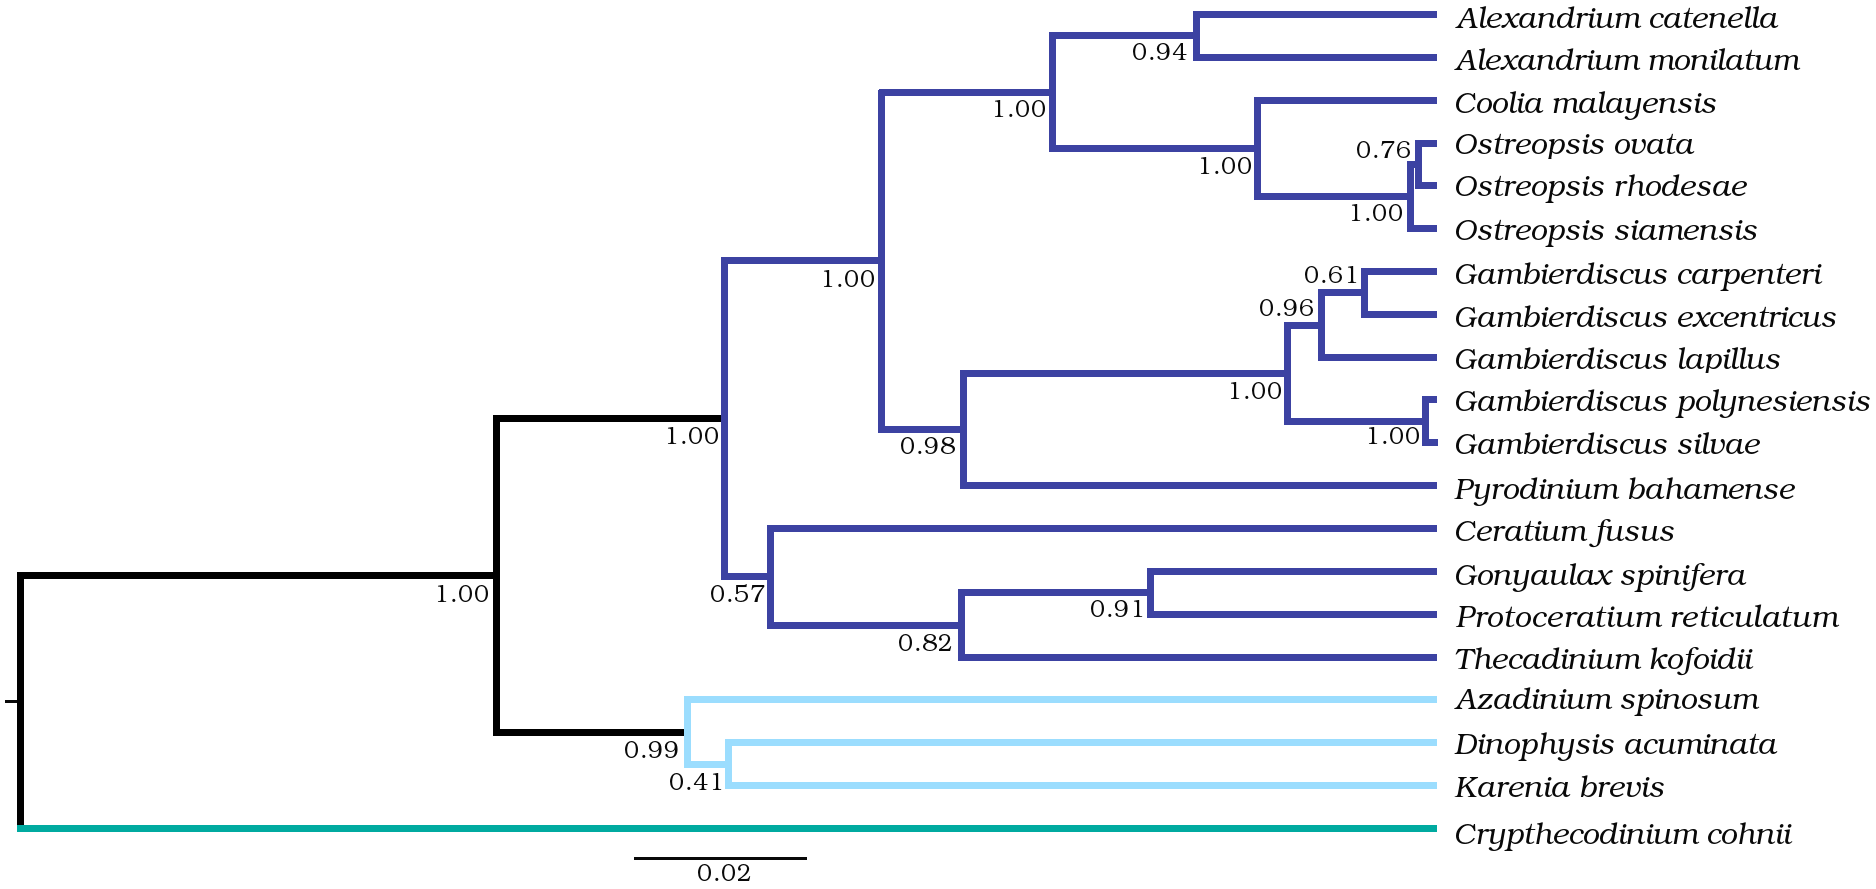
\includegraphics[scale=.25]{figures/Aug2_20-taxa-combined-fig_MCC_trees.png} 
\caption{Bayesian phylogenetic inference of Gonyaulacales species tree under the multipsecies coalescence with 62 single copy genes from 20 taxa. Gonyaulacales (\#16) in purple, outgroups (\#3) in light blue and taxa \textit{incertae sedis} (\#1) in teal. The scale represents number of substitutions per site.} 
\label{fig:SCmscBI}
\end{figure} 
\FloatBarrier

\newpage
\section{Discussion}
Phylogenetic inference of groups of microbial eukaryotes has been greatly enabled by the increasing amount of genetic data now available, including through large scale sequencing initiatives such as MMETSP \cite{keeling2014marine}.
However, the next obstacle lies in the methodology used for investigating the evolutionary relationship between these taxa, as the choice in data analysis method can impact the resultant phylogeny and conclusions drawn. 
Dinoflagellates are notorious for their extensive genomes with suspected whole or partial genome duplication and potential cDNA retro-insertion into the genome \cite{van2009florida.beauchemin2012dinoflagellate,slamovits2008widespread,hou2009distinct,lin2011genomic}. 
This causes unusually large gene copy numbers and extensive paralogy. 
With this in mind, the Gonyaulacales presented as an ideal challenge to test the process of paralog elimination for the methodology presented here as input for species inference.  
The authors hope the process presented here is transparent and reproducible for those with basic programming skills. 
Due to the size of their genomes and extensive paralogy the Gonyaulacales were chosen to test the methodology presented here.
We present a synopsis of the impact of model and data selection on the overall topology, while comparing commonly employed methodologies. \\
%AD: the following statement seems out of place. maybe you need to start a new paragraph about the problem of model misspecification? let's remember the well known words of George Box...all models are wrong
The authors are mindful that overparameterization as well as under parameterization can cause mis-specification for BI, if the inference is not in the Felsenstein zone. 
However under- compared to over-parameterization has been shown to have  more severe negatve impacts for inferring the an adequate approximation of the species tree \cite{lemmon2004importance}. 
%AD: path. does path sampling address model adequacy? i'm doubtful.
Hence integral to this study was the statistical comparison of concatenation versus MSC through stepping stone sampling as evidence for model parameter adequacy. 
The scripts which form the basis of this study are publicly available through github and the single copy genes used to infer the species evolution in this study, as well as the xml input and log files for the *BEAST runs, are available on zenodo. 
What follows is a discussion of the key methodological questions that this study sought to address, using the gonyalacales as a case study. 

%TODO refs, not sure if neede but were sent by Shauna:
% Disagreements in deeper branches in insect phylogenomic study which compared models - but used concat \cite{boussau2014strepsiptera}
% path sampling also penalises over-parameterization \cite{} because while bias decreses w/ #parameters, variance increases. So model \& it's parameters should hit the sweet spot between the two \cite{kelchner2007model} ... same for ss?

\subsection*{Quality of transcriptome assemblies.}
%Several studies have inferred the evolutionary relationship within the gonyaulacales as part of larger studies around the dinoflagellates, and as such the number of taxa from within the gonyaulacales is too limited to speculate on the families or clades within the order, e.g. \cite{shalchian2006combined,zhang2007three,saldarriaga2004molecular,hoppenrath2010dinoflagellate,murray2005improving}.
When using publicly available datasets, quality assessment is essential. 
Since the MMETSP datasets were made available, several studies have utilized a broader range of taxa to explore evolutionary stories involving the Gonyaulacales. 
However, these have relied on the assemblies supplied as part of the project. 
The stringency for quality trimming of RNA-seq libraries prior to assembly plays a role in the number of unique contigs recovered and the subsequent assembly quality of transcriptomes. 
Regarding the transcriptome assembly method, Cohen et al. evaluated the publicly available assemblies from MMETSP using BUSCO scores, compared to processing and re-assembly with Trinity \cite{cohen2018mmetsp}. 
Cohen et al. demonstrated that while the raw data available from the MMETSP project is an excellent resource, the assemblies available as part of the project are of a quality less than what can be achieved with current methods. 
Another factor in assembly quality is RNA-seq library processing prior to assembly, especially trimming. 
Commonly high stringency is favored, however MacManes (2014) found that this can be detrimental to the assembly and the quality cut off scores used in this study were based on the recommendation with that study \cite{macmanes2014optimal}.
In short, the trimming and assembly pipeline used for the assemblies available as part of MMETSP have become outdated and this is reflected in the quality comparison conducted by Cohen et al. 
To address this problem, trimming and assembly of RNA-seq libraries using Trimomatic and Trinity respectively were considered integral to the transcriptome assembly in this study.

\subsection*{Quantity of taxa in phylogenetic inference}
%eukaryotic deep lineages show evidence of rapid diversification \cite{he2016reducing} -- actually maybe find a different ref for this, they're kinda shite, which results in short internl brnaches which is the play ground for ILS.
% ---> \cite{degnan2006discordance} describes that methods which rely on democratic elucidation of species tree by most common gene tree are statistically predisposed to being wrong as anomatolous gene trees are likely with asymetric trees, and this holds true for any trees with 5 or more taxa (ie. if there are long and short branches). uses coalescence as example
Extensive coverage of taxa within the group of organisms examined is necessary to give useful insight into the evolutionary inter-taxon relationships.
Two concerning phenomena that can confound the veracity of the conclusion drawn from phylogenetic inference are incomplete lineage sorting (ILS) and long branch attraction (LBA). 
%AD: the following sentence doesn't make sense
The lack of adequate coverage is termed ILS and subject to postulated detrimental impact through bias on inferences \cite{heath2008taxon}. 
The impact of ILS on phylogenetic inferences has been explored through simulated datasets with a known species tree. 
Maddison and Knowles (2006) found that ILS can be overcome with an increase in genes rather than taxa due to the information retained in the signal from informative sites in the genes \cite{maddison2006inferring}. 
%AD: here it sounds like you're talking about limited taxon sampling, but this is the first place in the manuscript I've noticed it. Would be good to address this up front somewhere, especially given the important suggestion that having lots of genes can overcome limited taxon sampling.
So extrapolating from the simulation data studies available, a large number of genes should overcome the incomplete coverage of the families from the gonyaluacales and give an accurate representation of the evolutionary relationships despite the missing taxa. 
In contrast, LBA is exacerbated if ILS is present. 
LBA can arise if some species have disproportionately high substitution rates which causes the presence of long and short branches in the phylogenetic topology \cite{liu2014coalescent}. 
%AD: maybe cite something that previously described a dino radiation?
Short internal branches with long external branches are symptomatic of ancient lineage radiation, which is a characteristic commonly associated with the dinoflagellates. 
Under these conditions, concatenation methods are more likely to be mislead and fall prey to LBAs than MSC methods \cite{liu2014coalescent}.

\subsection*{Phylogenetic inference using ribosomal genes.}
\FloatBarrier 
Using LSU or SSU rDNA regions for phylogenetics is common practice, at times supplemented with a small number of other genes \cite{shalchian2006combined,zhang2007three,saldarriaga2004molecular,murray2005improving,hoppenrath2010dinoflagellate}. 
It is important to acknowledge that these represent the evolutionary history of highly conserved genes, which does not necessarily represent the species evolution and assuming their congruence is statistically inadequate \cite{degnan2009gene}.
%AD: maybe add something positive like "...and we have learned much from rDNA phylogeny" at the end of the sentence? alternatively it could go in a sentence below about how its still common practice
%LK: this ok?
Utilization of rDNA loci made sense when study designs were bound by sequencing and computational limitations, so they were a universally available proxy which was informative and continues to be commonly employed. 
With high throughput sequencing and high performance computing now commonly available, we are no longer restricted to the use of rDNA datasets as proxies for species evolution. 
Yet rDNA loci are still widely used for Gonyaulacales. 
%AD: would it be better to first compare different data with same method (e.g. rDNA concat vs scg concat) before describing different data & different method?
%you might even add \paragraph{} subheadings for "same data, different method" etc?
Comparing the topology from a rDNA ML inference with the single gene copy MSC phylogeny presented here (Fig. ~\ref{fig:tanglerDNA}) shows that most clades in both topologies were completely or very well supported. 
Within the genera \emph{Gambierdiscus} and \emph{Ostreopsis}, the species resolution differed between the two datasets. 
In several cases, the placement of sister taxa was incongruous between the two analyses. 
For example, the rDNA concatenation dataset places \emph{Ceratium} \& \emph{Gonyaulax} as well as \emph{Alexandrium} and \emph{Gambierdiscus} as sister taxa, while the single copy gene dataset under MSC places \emph{Gonyaulax} with \emph{Protoceratium} and \emph{Gambierdiscus} with \emph{Pyrodinium}. 
This is an example of how using rDNA segments as a proxy for species evolution can provide different results than an analysis of single-copy protein coding genes.

\begin{figure} 
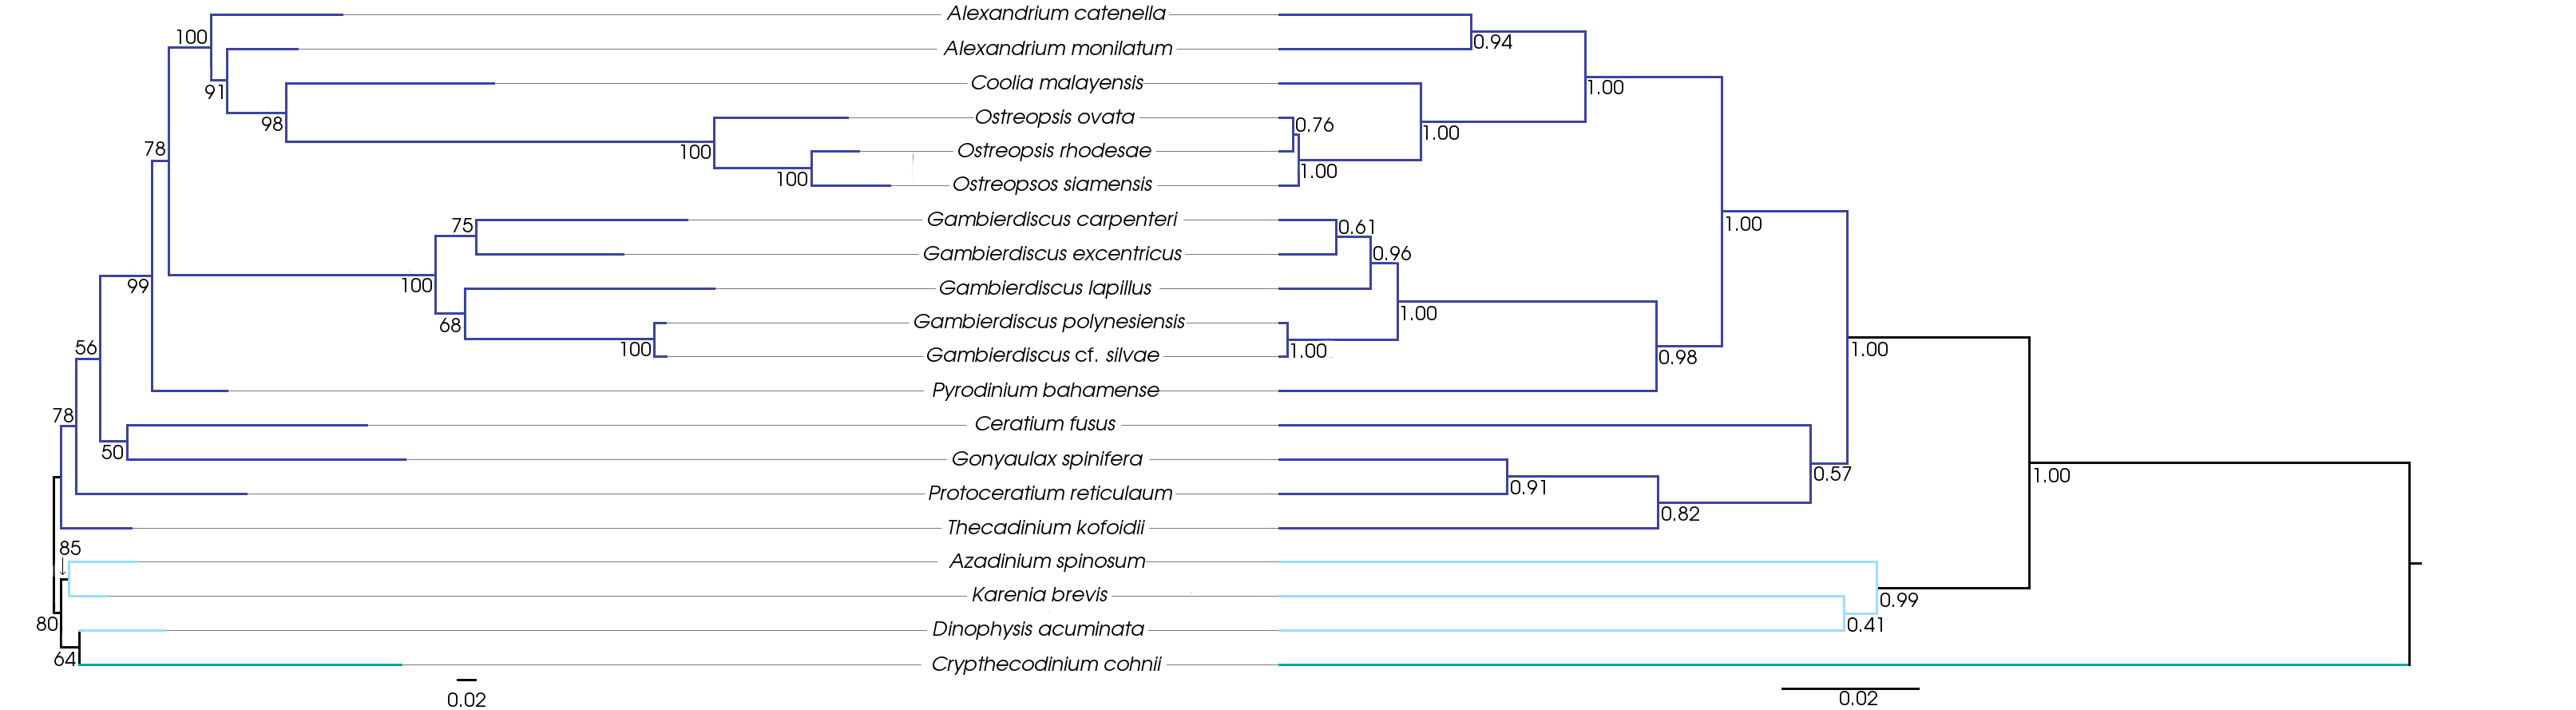
\includegraphics[scale=.2]{figures/MSC-BI_vs_rDNA-ML.png} 
\caption{Tanglegram showing the topological differences in phylogenies from (A) concatenated rDNA genes (SSU and D1-D3 LSU) infered with ML; and (B) MSC starbeast inference with 58 single copy genes. Gonyaulacales (\#16) in purple, outgroups (\#3) in light blue and taxa \textit{incertae sedis} (\#1) in teal.} 
\label{fig:tanglerDNA}
\end{figure} 
\FloatBarrier

\subsection*{Concatenating selected genes and using ML methods for species inference.}
\FloatBarrier
Concatenation of alignments coupled with running ML inference is a commonly used method as it is computationally un-intensive in comparison to BI methods. 
However as demonstrated by Kubatko et al. (2007) and Roche et al. (2015), this approach is error prone. 
%AD: i'm not sure what the 2nd half of the following sentence means. What is a homogenised deviation? Do you mean a uniformly random deviation? And the deviation is only acceptable in evolutionary rate, not topology? branch lengths? What is an "unrealistic predictor"? Do you mean it yields biased estimates? inaccurate?
Concatenation assumes uniform evolutionary history across genes, with a homogenised deviation possible - however as this is on the average evolutionary rate between the genes as input, it's still an unrealistic predictor across multi gene datasets. 
The combination of concatenation and ML for phylogentic inference can result in high bootstrap values for incorrectly resolved clades which overinflates confidence in the robustness of erroneous topologies \cite{degnan2009gene}. 
The application of concatenation in combination with ML is common practice in phylogenetic studies for gonyaulacoids  \cite{shalchian2006combined,zhang2007three,saldarriaga2004molecular,murray2005improving,hoppenrath2010dinoflagellate}.
We investigated whether use of a technique explicitly designed to handle multiple genes to estimate species trees would yield different results than concatenation and ML. 
%AD: the comment about rDNA seems confusing here. perhaps either expand on it or move it elsewhere.
A comparison between a BI inference under MSC compared to concatenated ML inference on the same single copy gene dataset shows differences in topology, albeit different when comparing to the rDNA dataset (Fig. ~\ref{fig:tangleconcatML}). 
The species resolution within the genera \emph{Alexandrium}, \emph{Gambierdiscus} and \emph{Ostreopsis} matches between the two inference methods. 
The major difference is of the \emph{Pyrodinium} placement, where the BI MSC approach places the genus sister to \emph{Gambierdiscus} while the concatenated ML approach places it with \emph{Gonyaulax} and \emph{Protoceratium}. 
Further, the deeper branches of the phylogenies differ. 
The BI MSC method clusters \emph{Ceratium}, \emph{Gonyaulax}, \emph{Protoceratium} and \emph{Thecadinium} as a clade, while the concatenated ML approach clusters \emph{Gonyaulax}, \emph{Protoceratium} and \emph{Pyrodinium} as a clade to which \emph{Thecadinium} and then \emph{Ceratium} feature as ancestral genera. 

\begin{figure} 
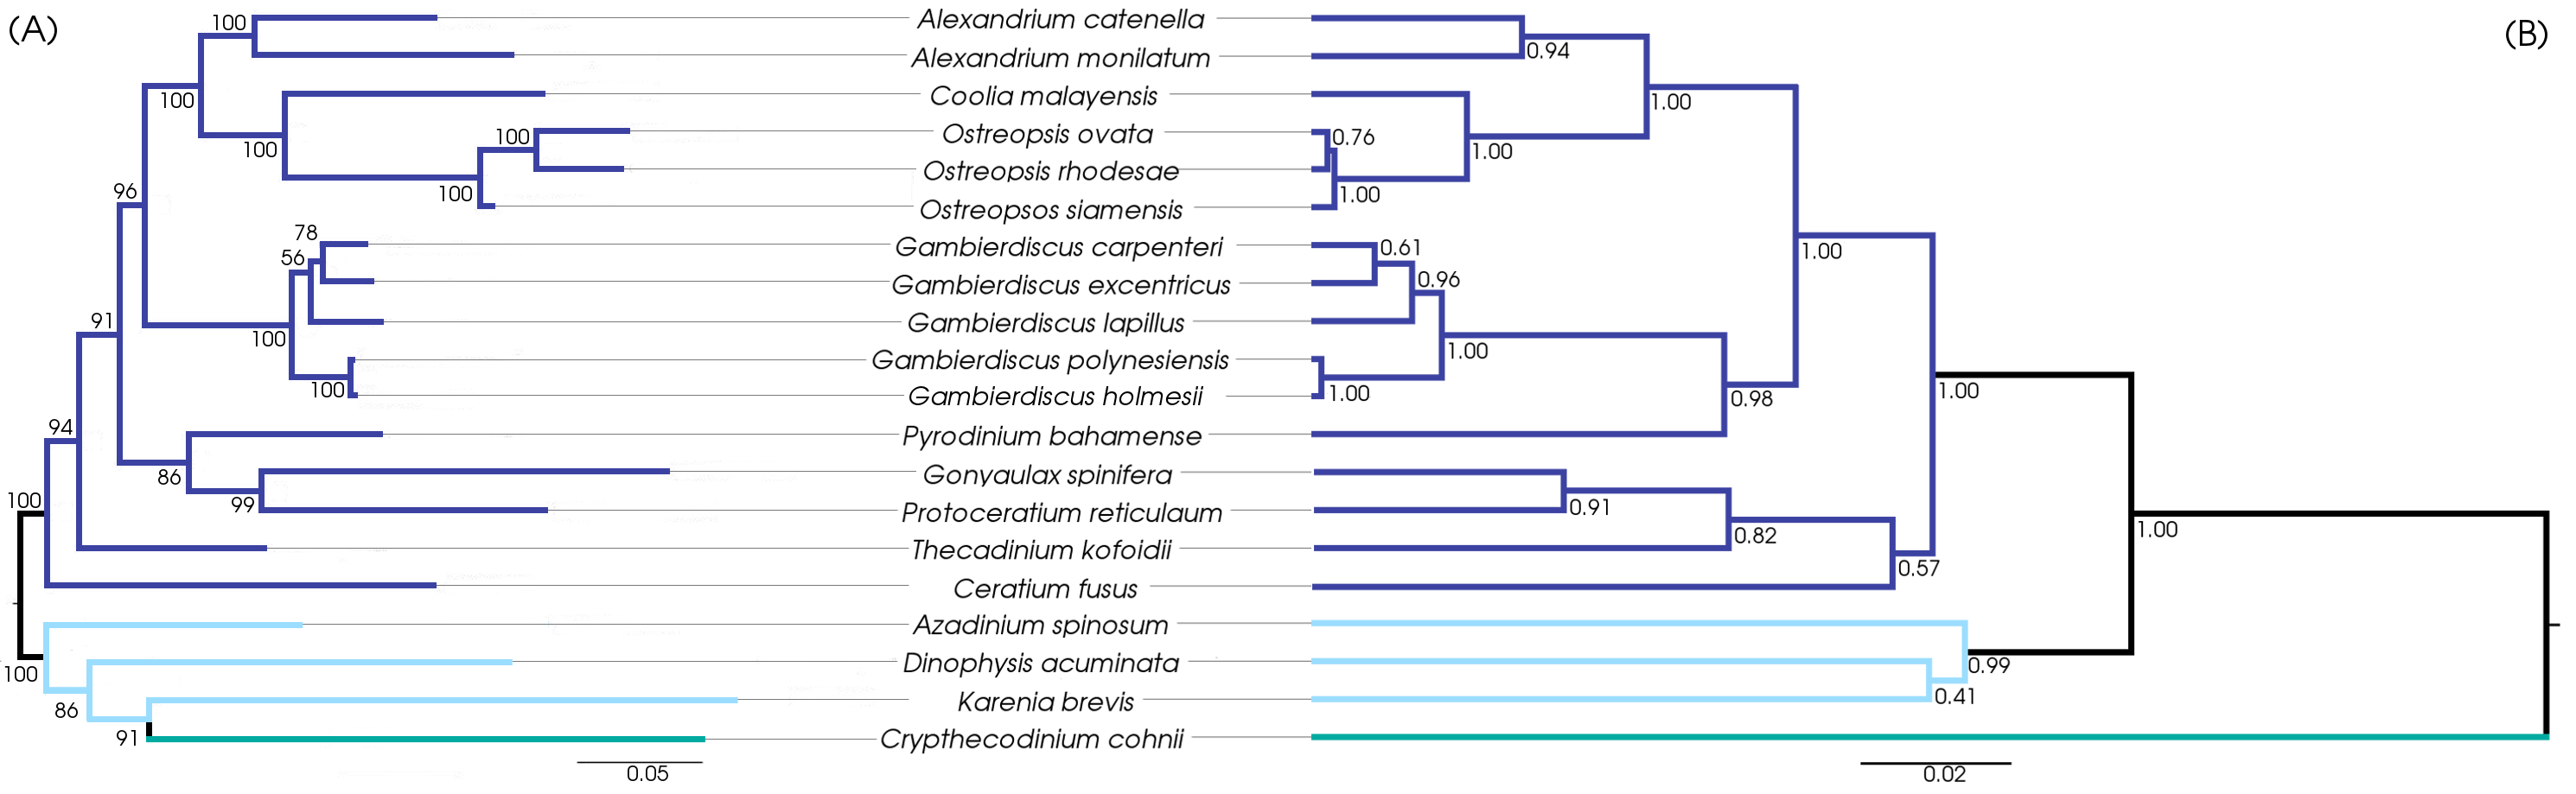
\includegraphics[scale=.2]{figures/MSC-BI_vs_singlecopy-concat-ML.png} 
\caption{Tanglegram showing the topological differences in phylogenies with same 58 single copy gene alignments as input. (A) concatenated ML inference; and (B) MSC starbeast inference. Gonyaulacales (\#16) in purple, outgroups (\#3) in light blue and taxa \textit{incertae sedis} (\#1) in teal.} 
\label{fig:tangleconcatML}
\end{figure} 
\FloatBarrier

\subsection*{Concatenating selected genes and using BI methods for species inference.}
\FloatBarrier
Even within a BI framework, while more robust than when used in conjunction with ML, concatenation can introduce a number of errors. 
Under simulated datasets, even under the coalescent methods, the species tree topology is inaccurate when concatenation is used \cite{kubatko2007inconsistency}. 
Further to that, the PP values tend to be overestimated for concatenation \cite{suzuki2002overcredibility}. 
Theoretically for the gonyaluacales, and taxa prone to paralogy and convoluted evolutionary histories, MSC is a preferable approach to concatenation as MSC is more robust to ILS \& LBA artefacts \cite{liu2014coalescent}. 
To test this theory, the single copy gene dataset was run with BI both under MSC and with concatenation (Fig. ~\ref{fig:tangleconcatBI}). 
We then used a statistical framework to compare the two model approaches to verify the veracity of model adequacy through stepping stone sampling. 
PATH sampling is an adequate method for objectively comparing the model parameters for relaxed clock models while penalizing for over-parameterization \cite{baele2012accurate}. %TODO same for ss?
The valuex XXX %TODO whatever the hell the PATH sampling results are
%TODO topology comparison here 
The resolution of \textit{Alexandrium}, \textit{Coolia} and \textit{Ostreopsis} was identical between the two methods. 
Further, the species resolution within the genera \textit{Gambierdiscus} and \textit{Ostreopsis} was also identical. 
Differences were found in the topology, in that \textit{Pyrodinium} clustered with \textit{Gambierdiscus} in the MSC analysis, while for concatenation this genus clusters with \textit{Gonyalax} and \textit{Protoceratium}. 
Further, in the MSC analysis \textit{Ceratium}, \textit{Gonyalax}, \textit{Protoceratium} and \textit{Thecadinium} form their own clade while with concatenation, \textit{Ceratium} and \textit{Thecadinium} are ancestral genera to the rest of the Gonyaulacales. 

  
%with concatenation, coalescent methods still commonly return inaccurate species tree resolutions \cite{kubatko2007inconsistency} 
%Suzuki 2002 shows that PP is overestimated when concatenation is used
%TODO \cite{baele2012accurate} for Path sampling as accurate model assessment method for relaxed clock models... are any improper priors used? PS may not be able to sample from the prior %TODO see if ok for ss

% MSC robust for both ILS & LBA unlike concat <3 \cite{liu2014coalescent} ; example from water lillies with same phenomenon \cite{liu2014coalescent}

%TODO CHeck again after ss sampling is complete and also if run0 is posterior
\begin{figure} 
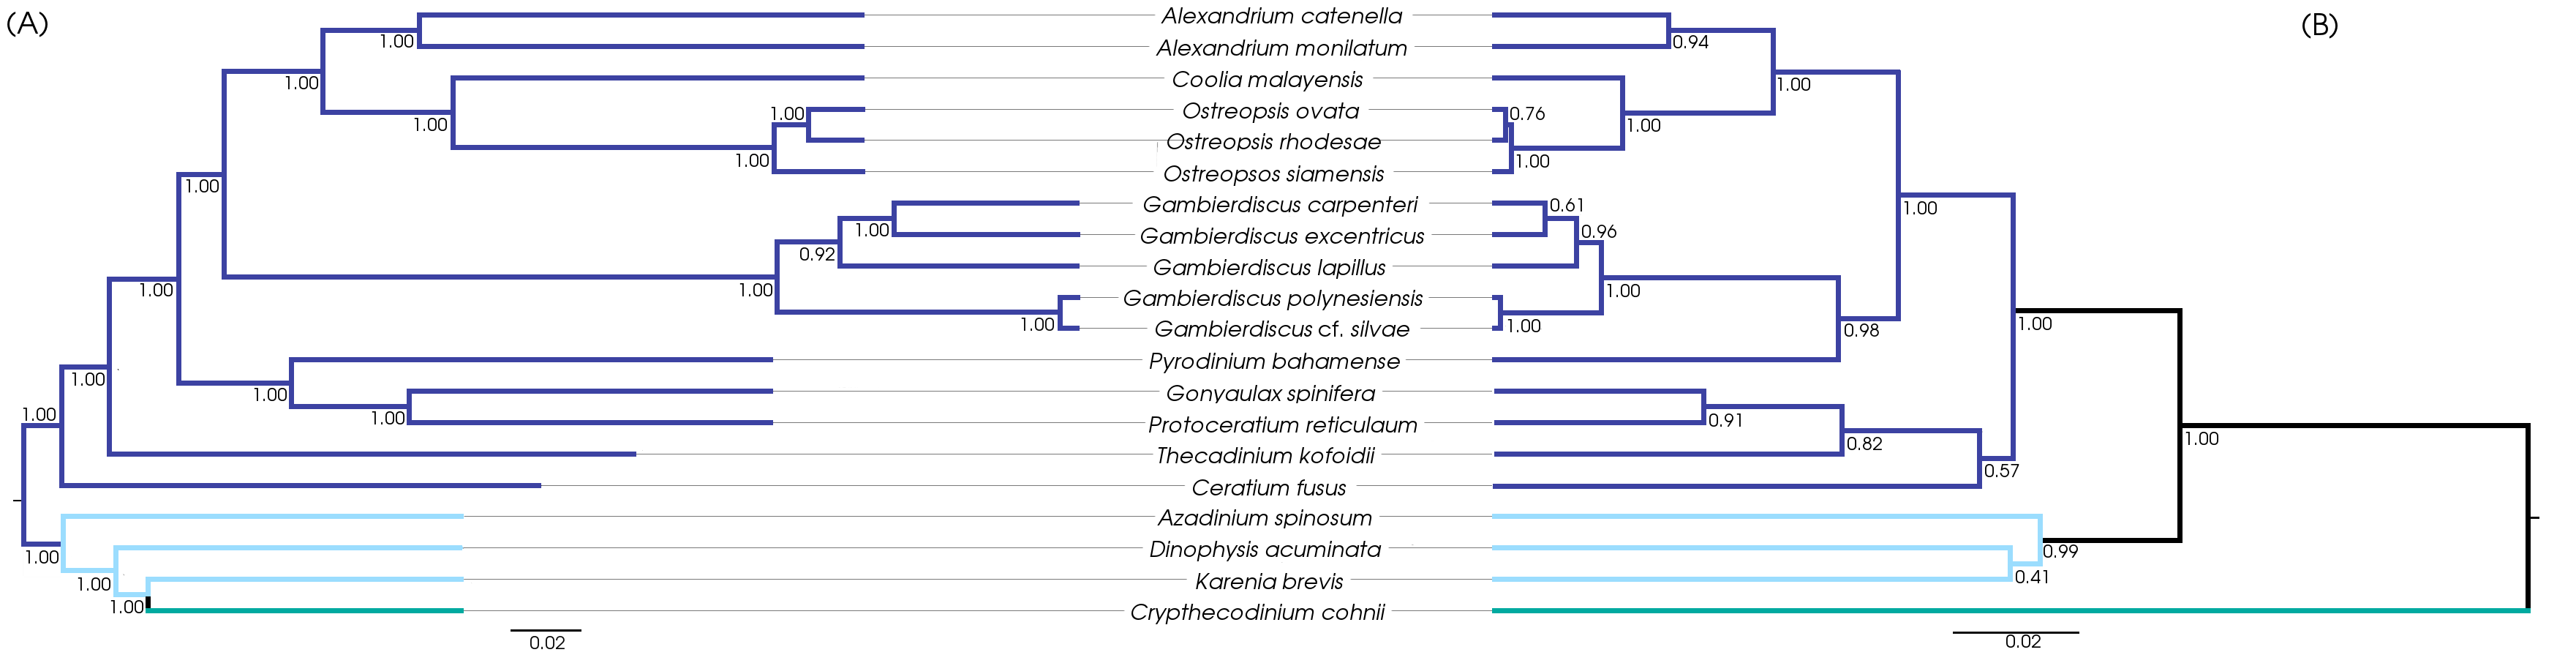
\includegraphics[scale=.18]{figures/SC-MSC-BI_vs_SC-concat-BI.png} 
\caption{Tanglegram showing the topological differences in phylogenies with same 58 single copy gene alignments as input. (A) concatenated beast2; and (B) inference MSC starbeast inference. Gonyaulacales (\#16) in purple, outgroups (\#3) in light blue and taxa \textit{incertae sedis} (\#1) in teal.} 
\label{fig:tangleconcatBI}
\end{figure} 
\FloatBarrier

\subsection*{Selection of paralogs to infer species evolution.}
%\cite{yang2014orthology} orthologue extr method which means good discussion on problems with wrong selection
%\cite{degnan2009gene} some bullshit bout paralogs in soy bean
Selection of paralogs for species inference is highly problematic as it compares an arbitrarily divergent gene history as input. 
%sm: Need to explain and unpack. Ie, Under some circumstances, genes that are not orthologous, but are instead the result of subsequent gene duplication events within species (ie paralogous) can be mistaken for one another. This causes incorrect phylogenetic inference due to XYZ.  This problem is particularly apparent in species in which many genes exist in multiple copies in the genome, and for which multi-gene families are very common. In dinoflagellates.... In this study, this issue was addressed by
%LK: this was supposed to be apparent from the introduction. Does it really need to be explained again
This problem is particularly prevalent in the dinoflagellates and Gonyaulacales due to extensive paralogy from gene duplication. 
This study sought to address the issues arising from paralog comparison by isolating single copy genes, based on the BUSCO software output. 
As this software utilizes lineage specific hmmer libraries designed to target single copy genes, and the output distinguishes between single copy genes and duplications, it presents a method for reliably screening for single copy genes for phylogenomics \cite{waterhouse2017busco}.
Only one other study by Price et al. (2017) sought to address the issue of parology within the gonyalacales, by selecting single genes as input. 
However there are several issues with the study presented by Price et al \cite{price2017robust}. 
The assemblies used are from the MMETSP project, which employed outdated assembly methods as mentioned previously, and hence could present single copy genes which are instead hybrids of paralogs. 
Further, the methodology for identifying and selecting the single copy genes was not described in the publication and is not available upon request. 
Contact with the author established that there was no documentation for the commands that the authors executed, so no record of how the genes were attained was available. 
Hence it was impossible to compare the parameters that went into identifying and screening for single copy genes and it was not possible to scrutinize or reproduce the study.

Lastly, the genes were concatenated and the evolutionary relationships were inferred using ML. 
While the bootstraps are well supported, this could very well be due to the methodology problems outlined in previous sections.
The difference in topology between inferences presented by Price et al. and this study, is lies in the organization of sister taxa (Fig. ~\ref{fig:tangle}). 
Price et al. place \emph{Alexandrium} spp. as the closest genus to \emph{Gambierdiscus}, while this study places \emph{Pyrodinium} as sister. 
As some \emph{Gambierdiscus} spp. produce polyketide toxins which cause ciguatera fish poisoning, establishing the close relations to \emph{Gambierdiscus} is important for investigating the toxin evolution \cite{pawlowiez2014transcriptome}.
The placement of the genus \emph{Azadinium} is equally as divergent as Price et al. place this genus as part of the gonyaulacales, while this study firmly places this genus as an outgroup with \emph{Dinophysis} spp. and \emph{Karenia} spp.
As \emph{Azadinium} spp. also produce polyketide toxins that cause azaspiracid shellfish poisoning, their placement is important for investigating polyketide toxin evolution \cite{meyer2015transcriptomic}.
\FloatBarrier 
\begin{figure} 
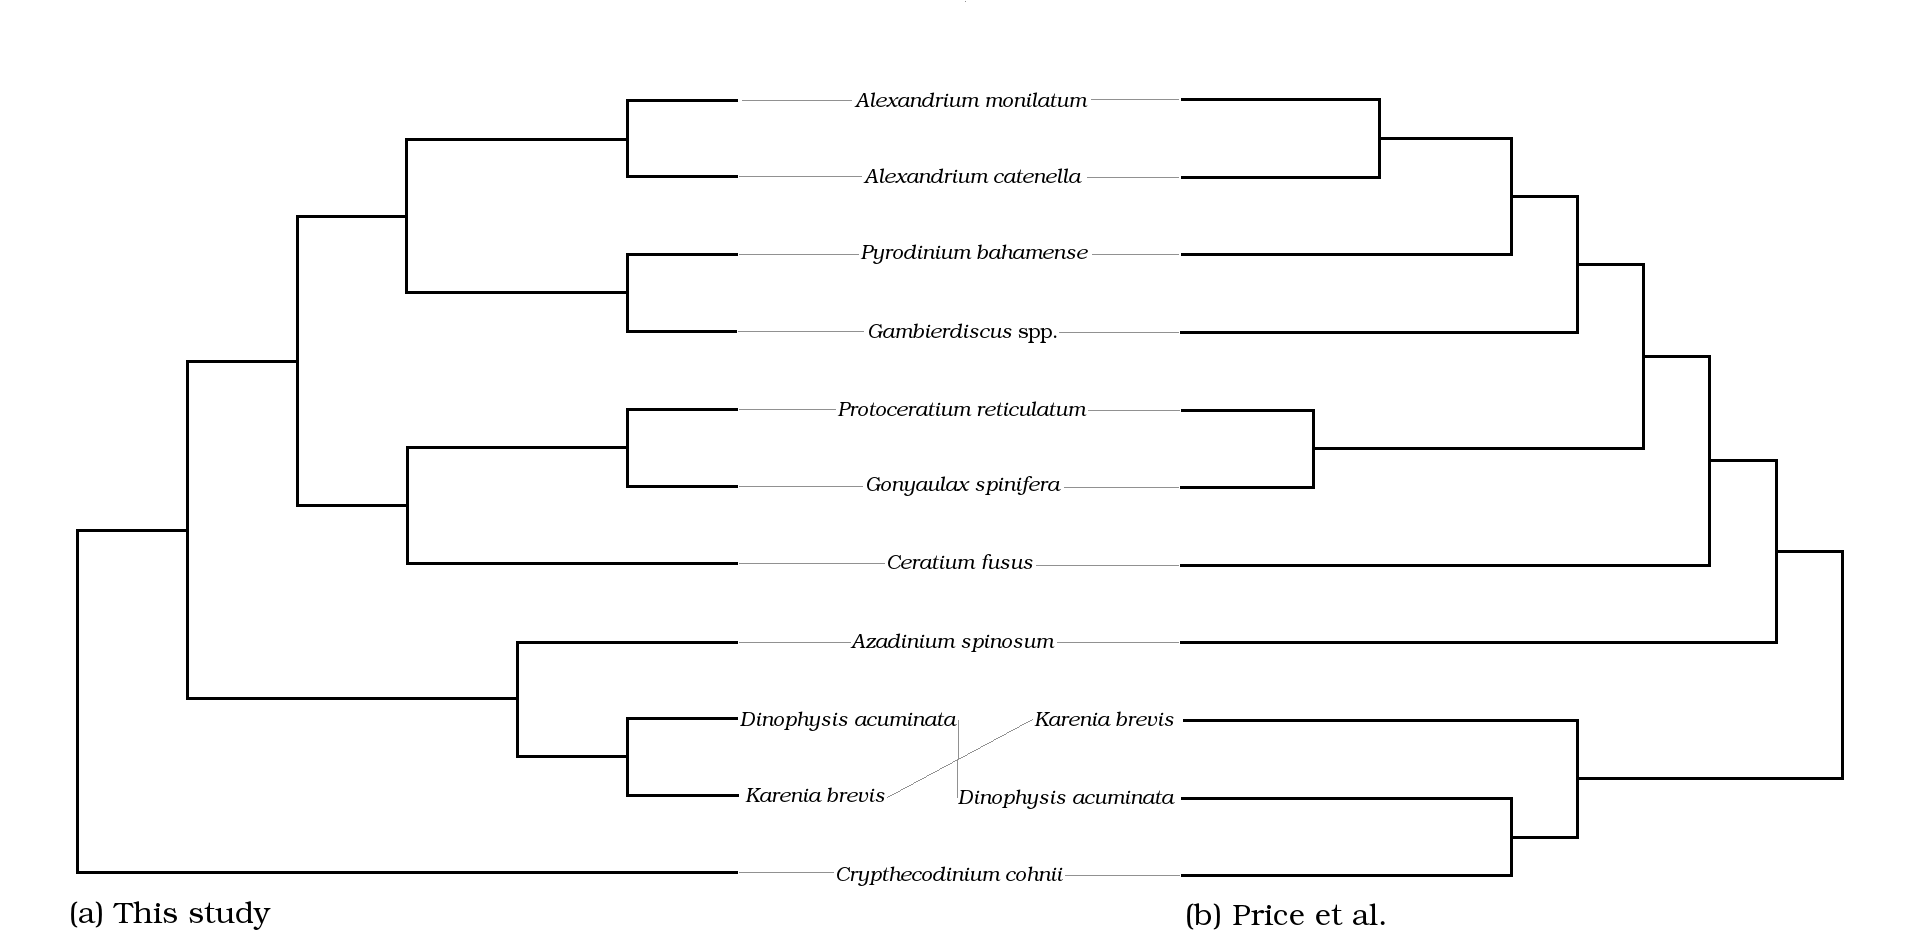
\includegraphics[scale=.23]{figures/Price-comparison.png} %TODO include bootstraps
\caption{Tanglegram of topology presented in this study (a); and Price et al. (2017) (b). Taxa uncommon to both studies not shown.} 
\label{fig:tangle}
\end{figure} 
\FloatBarrier
In this study, we utilised the BUSCO output which screens for and verifies single copy genes for input into species tree inference, a purpose which was suggested as ideal by the authors of the software \cite{simao2015busco}. 

\subsection*{Limitations of study}
In the previous section we identified potential problems with common approaches to species inference in the literature, and in particular for the Gonyaulacales. 
We then sought to demonstrate that our methodology is more robust for addressing these problems. 
However we do not imply that this study is not fraught with potential methodological errors. 
We aim to present avenues for improvement on routine methods, delivering a simple \& reproducible way to access these methods and to demonstrate the impact the method and data selections have on phylogenetic inference. 
What follows is the identification of issues with the approach presented in this study, which the authors hope will be improved upon by subsequent studies. 
\paragraph*{Trimming of RNA seq libraries.} The cut off values chosen for this study are based on the recommendations of MacMannes (2014) for optimal transcript discovery. 
However the recommendations are based on the efficacy of cut off values for a mouse embryonic stem cell RNA-seq library, which may not be an adequate model for dinoflagellates. 
This could confound the difference between single copy genes and sequencing artifacts.
\paragraph*{Assembly parameters.}
Trinity was chosen as the assembler for this study based on the findings of Honaas et al. (2016), in which Trinity was one of the top performing assemblers for \textit{de novo} transcriptomes as tested with \textit{Arabidopsis thaliana}. 
While this plant model has similar genetic features to dinoflagellates, the conclusion of adequate comparison may be flawed.
Further, Trinity performed well for identifying isoforms of genes and excelled at assembling highly expressed genes \cite{honaas2016selecting}.
Conversely, Cerveau et al. (2016) found that Trinity, CLC Bio and IDBA-Tran assemblies all contain bioinformatic artifacts. 
Using a combination of all three assemblers yielded a final assembly closer to biological reality than any individual assembler, when no reference genome is available \cite{cerveau2016combining}.
As this study uses Trinity exclusively, it is subject to the bioinformatic errors found by Cerveau et al. (2016) which could affect downstream analysis.
\paragraph*{Contamination of other taxa.} 
The 650+ RNA extract submission to MMETSP was from a large number of investigators and low level contamination is inherent in the project's dataset \cite{keeling2014marine}. 
As the cultures tested in all the studies contributing to this dataset were not axenic, contamination could be bacterial or eukaryotic in nature. 
However the likely divergence from genes selected from bacterial contamination would likely be very obvious in the inferece.
\paragraph*{No representative genome for comparison.} 
Without a guided genome comparison, it is difficult to extrapolate on the assembly adequacy and whether the genes selected are single copies, or mis-assemblies of paralogs.
\paragraph*{Different methods for RNA-seq.} 
Three different approaches for RNA-seq library generation were employed for the libraries used in this study, the MMETSP taxa were sequences on HiSeq platform with 50bp inserts; while all other taxa were sequenced on the NextSeq platform with 75bp or 150bp inserts. 
The incongruity between sequencing methods may cause divergent accuracy in single copy gene coverage for sequencing.  
\paragraph*{Total evidence phylogenetics.}
The method presented here purely considers the information contained in the genetic aspect of the organsims examined. 
Morphological characters and fossil dates can add another dimension to the phylogenetic resolution of taxa placement and put the evolution within a relative time frame \cite{gavryushkina2017bayesian}.  

\newpage
\section{Conclusion}
With the public accessibility of large data sets, the focus needs to shift to the methodology used to analyze them. 
This study presents a robust methodology BI MSC based species inference. 
The scripts process RNA-seq libraries through assembly, single copy gene selection to alignment for phylogenetic species inference. 
As a case study exemplifying organisms rife with paralogs and ancient lineages, the Gonyaulacales were selected. 
The resulting phylogeny shows a well resolved, well supported and statistically sound inference of the Gonyaulacales evolution. 
This was then compared to phylogenies inferred from commonly utilized methods in the literature, and issues arising from these methods were discussed. 
By presenting a statistically rigorous methodology and demonstrating how this overcomes common problems faced in phylogenetic studies, we hope that the use of reproducible, open-access processing of large data-sets such as the MMETSP database becomes the standard.  
\newpage

\section{Acknowledgments}
The GVL section of this study was conducted inside the National eResearch Collaboration Tools and Resources (NeCTAR) research cloud, an initiative by the National Research Infrastructure for Australia (NCRIS).
Gratitude to the Stanley Watson foundation, the Linnaean Society of New South Wales, and the ABRS National Taxonomy Research Student Travel Bursary for funding A. L. Kretzschmar's attendance at the Molecular Evolution workshop at the Marine biological laboratory, Woods Hole, MA, USA.
Shout out to the Taming the BEAST organizers \& fellow attendees for a most illuminating workshop in February 2017 on BEAST methodology, and to Geneious for subsidizing A. L. Kretzschmar's attendance fee.
Thank you to Dr. Tim Kahlke for running Interproscan for transcriptome analysis. 
The transcriptomic sequencing was funded by  an ARC Future Fellowship to S. Murray.
A. L. Kretzschmar's PhD stipend was funded through a UTS Doctoral scholarship.
\section{Supplementary material}
\FloatBarrier
\begin{table}
\caption{Table S1: Culturing conditions for species processed for this study.}
%\label{tbl:strainTable}
\begin{tabular}{ | p{3cm} | p{2.5cm} | p{1.5cm} | p{5.3cm} |}
\hline
\textbf{Species} & \textbf{Strain}& \textbf{Temp} & \textbf{Source location} \\
%\hline
%\textit{Coolia malayensis}&MAB&& \\
\hline
\textit{Gambierdiscus carpenteri}&UTSMER9A&17&Merimbula, AU\\
\hline
\textit{Gambierdiscus lapillus}&HG4&27&Heron Island, AU\\
\hline
\textit{Gambierdiscus polynesiensis}&CG15&27&Rarotonga, COK\\
\hline
\textit{Gambierdiscus} cf. \textit{silvae}&HG5&27&Heron Island, AU\\
\hline
%\textit{Ostreopsis ovata}&HER27&&\\
%\hline
%\textit{Ostreopsis rhodesae}&HER26&&\\
%\hline
%\textit{Ostreopsis siamensis}&BH1&&\\
%\hline
\textit{Thecadinium} cf. \emph{kofoidii}&THECA&18&Gordons bay, Sydney, AU\\
\hline
\end{tabular}
\end{table}
\FloatBarrier

\begin{longtable}{  | p{3.5cm} |p{2.2cm} | p{1.8cm} | p{1.8cm} | p{1.8cm} | p{3cm} |}
\caption{Table S2: Transcriptomes used for study along including strain ID, source and BUSCOv2 information. MMETSP abbreviation for marine Microbial eukaryotic transcriptome sequencing project, by Moore Foundation.}\\
\hline
%\label{tbl:Transcriptomes}
%\textbf{Family}&
\textbf{Species}&\textbf{Strain}&\textbf{complete BUSCOs}&\textbf{single complete BUSCOs}&\textbf{fragmented BUSCOs}&\textbf{Source}\\
\hline
 \multicolumn{6}{| c |}{Gonyaulacales transcriptomes}\\
    \hline
\emph{Alexandrium catenella}&OF101&110&74&3&MMETSP0790 \citep{keeling2014marine}\\
        \hline
\emph{Alexandrium monilatum}&JR08&107&74&3&MMETSP0093 \citep{keeling2014marine}\\
        \hline
\emph{Ceratium fusus}&PA161109&121&81&4&MMETSP1074 \citep{keeling2014marine}\\
        \hline
\emph{Coolia malayensis}&MAB&138&100&1&(Verma 2018, in prep)\\
\hline
\emph{Crypthecodinium cohnii}&Seligo&126&98&0&MMETSP0326\_2 \citep{keeling2014marine}\\
        \hline
\emph{Gambierdiscus carpenteri}&UTSMER9A&101&83&2&This study\\
\hline
\emph{Gambierdiscus excentricus}&VGO790&88&83&4&\cite{kohli2017role}\\
        \hline
\emph{Gambierdiscus lapillus}&HG4&141&98&2&This study\\
        \hline
\emph{Gambierdiscus polynesiensis}&CG15&104&81&3&This study\\
        \hline
\emph{Gambierdiscus} cf. \emph{silvae}&HG5&134&87&2&This study\\
        \hline
\emph{Gonyaulax spinifera}&CCMP409&83&53&2&MMETSP1439 \citep{keeling2014marine}\\
        \hline
\emph{Ostreopsis ovata}&HER27&132&99&2&(Verma 2018, in prep)\\
     \hline
\emph{Ostreopsis rhodesae}&HER26&131&98&1&(Verma 2018, in prep)\\
     \hline
\emph{Ostreopsis siamensis}&BH1&132&98&1&(Verma 2018, in prep)\\
     \hline
\emph{Protoceratium reticulatum}&CCCM535=CCMP1889&108&72&5&MMETSP0228 \citep{keeling2014marine}\\
    \hline
\emph{Pyrodinium bahamense}&pbaha01&119&897&2&MMETSP0796 \citep{keeling2014marine}\\
        \hline
\emph{Thecadinium} cf. \emph{kofoidii}&THECA&93&70&5&This study\\
 \hline
 \multicolumn{6}{| c |}{Outgroup transcriptomes}\\
 \hline
 \emph{Azadinium spinosum}&3D9&1.8&81&4&MMETSP1036\_2 \citep{keeling2014marine}\\
        \hline
\emph{Dinophysis acimunata}&DAEP01&117&74&2&MMETSP0797 \citep{keeling2014marine}\\
        \hline
\emph{Karenia brevis}&CCMP2229&115&85&2&MMETSP0030 \citep{keeling2014marine}\\
    \hline
\end{longtable}
\FloatBarrier
%families, sections which was taken out:Ceratiaceae,Crypthecodiniaceae,Gonyaulacaceae,Protoceratiaceae,Dinophysiaceae,Dinophyceae incertae sedis,Gymnodiniales

\begin{longtable}{  | p{3cm} |p{3cm} |  p{3cm} | }
\caption{Table S3: Accession numbers for ribosomal DNA sequences used for Fig. ~\ref{fig:rdna}. Sequences sourced from NCBI, except accesion numbers with '$\ast$' sourced from the Silva database. Genes not publically available are denoted by '-'.}\\
\hline
%\label{tbl:Transcriptomes}
%\textbf{Family}&
\textbf{Species}&\textbf{SSU seq.}&\textbf{D1-D3 LSU seq.}\\

\hline
 \multicolumn{3}{| c |}{Gonyaulacales taxa}\\
 \hline
\emph{Alexandrium catenella}&AB088286&AB088238\\
        \hline
\emph{Alexandrium monilatum}&AY883005&-\\
        \hline
\emph{Ceratium fusus}&AF022153&AF260390\\
        \hline
\emph{Coolia malayensis}&HQ897279$\ast$&KX589143\\
\hline
\emph{Crypthecodinium cohnii}&M64245&-\\
        \hline
\emph{Gambierdiscus carpenteri}&EF202908&EF202938\\
\hline
\emph{Gambierdiscus excentricus}&GETL01000157$\ast$&HQ877874\\
        \hline
\emph{Gambierdiscus lapillus}&KU558930&-\\
        \hline
\emph{Gambierdiscus polynesiensis}&EF202907&This study\\
        \hline
\emph{Gambierdiscus} cf. \emph{silvae}&This study&this study\\
        \hline
\emph{Gonyaulax spinifera}&AF022155&DQ151558\\
        \hline
\emph{Ostreopsis ovata}&AF244939&KJ781420\\
     \hline
\emph{Ostreopsis rhodesae}&KX055855&KX055845\\
     \hline
\emph{Ostreopsis siamensis}&KX055868&HQ414223\\
     \hline
\emph{Protoceratium reticulatum}&AF274273&EF613362\\
    \hline
\emph{Pyrodinium bahamense}&AY456115&AB936757\\
        \hline
\emph{Thecadinium} cf. \emph{kofoidii}&AY238478&KT371445\\
 \hline
\multicolumn{3}{| c |}{Outgroup taxa}\\
    \hline
  \emph{Azadinium spinosum}&JN680857&JN165101\\
        \hline
\emph{Dinophysis acimunata}&AJ506972&EF613351\\
        \hline
\emph{Karenia brevis}&EF492504&AY355458\\
\hline
\end{longtable}
\FloatBarrier

\newpage
\bibliographystyle{acm}
\bibliography{gonya.bib}

\end{document}